\documentclass{article}

\usepackage{fullpage}
\usepackage{amsmath}
\usepackage{textcomp}

\usepackage{tikz}

\usepackage{fancyhdr}
\pagestyle{fancy}
\renewcommand{\headrulewidth}{0pt}
\cfoot{\sc Page \thepage\ of \pageref{end}}

\begin{document}

{\large \noindent{}University of Toronto at Scarborough\\
\textbf{CSC A67/MAT A67 - Discrete Mathematics, Fall 2015}}

\section*{\huge Exercise \#3: Counting and Probability}

{\large Due: October 2, 2015 at 11:59 p.m.\\
This exercise is worth 3\% of your final grade.}\\[1em]
\textbf{Warning:} Your electronic submission on MarkUs affirms that this exercise is your own work and no
one else's, and is in accordance with the University of Toronto Code of Behaviour on Academic Matters,
the Code of Student Conduct, and the guidelines for avoiding plagiarism in CSC A67/MAT A67.\\[1ex]
This exercise is due by 11:59 p.m. October 2. Late exercises will not be accepted.\\[1ex]
\renewcommand{\labelenumi}{\arabic{enumi}.}
\renewcommand{\labelenumii}{(\alph{enumii})}
\begin{enumerate}
\item Compute\marginpar{[2]} the coefficient of $x^8$ in the expansion of $(3x-2)^{13}$.
\item A\marginpar{[3]} computer generates a random four-digit string in the symbols A, B, C, \ldots, Z.
	\begin{enumerate}
	\item How many such strings are possible?
	\item What is the probability that the random string contains no vowels (A, E, I, O, U)?
	\end{enumerate}
\item If\marginpar{[2]} you roll two six-sided dice, what is the probability of rolling a 7 (as their sum)?
\item If\marginpar{[2]} you roll two four-sided dice (with numbers 1, 2, 3, and 4), what is the probability of rolling a 5?\\[1ex]
\textit{(Just for fun: can you draw a four-sided die?)}
\item A rook\marginpar{[5]} is a chess piece that attacks other pieces by moving horizontally or vertically. How many ways can you place $n>0$ rooks on a chessboard so that no two attack each other, if
	\begin{enumerate}
	\item all the rooks are identical?
	\item you have 4 wooden and 4 marble rooks?
	\item all the rooks are different?
	\end{enumerate}
For example, here are 5 nonattacking rooks on a chessboard:
\begin{center}
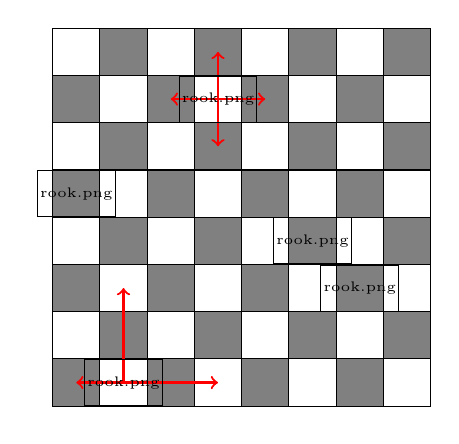
\begin{tikzpicture}[scale=0.6]
\foreach \x in {0,...,7}
	\foreach \y in {0,...,7}
		\node[draw,rectangle,minimum size=0.6cm] at (\x cm,\y cm) {};
\foreach \x in {0,2,...,7}
	\foreach \y in {0,2,...,7}
		\node[draw,rectangle,minimum size=0.6cm,fill=gray] at (\x cm,\y cm) {};
\foreach \x in {1,3,...,7}
	\foreach \y in {1,3,...,7}
		\node[draw,rectangle,minimum size=0.6cm,fill=gray] at (\x cm,\y cm) {};

\pgfdeclareimage[height=0.6cm]{rook}{rook.png};

\draw[->,red,thick] (1cm,0cm) -- (3cm,0cm);
\draw[->,red,thick] (1cm,0cm) -- (0cm,0cm);
\draw[->,red,thick] (1cm,0cm) -- (1cm,2cm);

\draw[->,red,thick] (3cm,6cm) -- (3cm,7cm);
\draw[->,red,thick] (3cm,6cm) -- (4cm,6cm);
\draw[->,red,thick] (3cm,6cm) -- (3cm,5cm);
\draw[->,red,thick] (3cm,6cm) -- (2cm,6cm);

\node at (1cm,0cm) {\pgfuseimage{rook}};
\node at (3cm,6cm) {\pgfuseimage{rook}};
\node at (0cm,4cm) {\pgfuseimage{rook}};
\node at (5cm,3cm) {\pgfuseimage{rook}};
\node at (6cm,2cm) {\pgfuseimage{rook}};
\end{tikzpicture}
\end{center}
\end{enumerate}
\hrulefill\\
\noindent[Total: 14 marks]\label{end}

\end{document}